\begin{table}[!h]
    \begin{center} 
        \begin{tabular}{|p{1.8cm}||p{1.6cm}|p{1.6cm}|p{1.6cm}|p{1.6cm}|p{1.6cm}|p{1.6cm}|}
            \hline
                \multicolumn{6}{|c|}{Task 1 - TDD} \\
            \hline
                Metric & Min & Max & Mean & Median & Std \\
            \hline
                QLTY & 73 & 96 & 81.12 & 77.77 & 10.73 \\
                PROD & 72 & 96 & 83 & 82 & 10 \\
                TEST & 8 & 10 & 9.5 & 10 & 1 \\
                CYC & 21 & 28 & 24.75 & 25 & 2.87 \\
                COG & 14 & 25 & 19 & 18.5 & 4.69 \\
                LOC & 154 & 195 & 167 & 159.5 & 18.95 \\
            \hline
        \end{tabular}
        \caption{\label{tab_dv_t1_tdd}Dependent variables' statistics in task 1 for the \tdd group}
    \end{center}
\end{table}

\begin{table}[!h]
    \begin{center} 
        \begin{tabular}{|p{1.8cm}||p{1.6cm}|p{1.6cm}|p{1.6cm}|p{1.6cm}|p{1.6cm}|}
            \hline
                \multicolumn{6}{|c|}{Task 1 - NO-TDD} \\
            \hline
                Metric & Min & Max & Mean & Median & Std\\
            \hline
                QLTY & 65.55 & 82 & 75.35 & 78.77 & 7.43 \\
                PROD & 56 & 84 & 76 & 80 & 11.66 \\
                TEST & 0 & 12 & 3.8 & 0 & 5.49 \\
                CYC & 12 & 18 & 15.6 & 16 & 2.19 \\
                COG & 9 & 17 & 14 & 15 & 3 \\
                LOC & 74 & 157 & 111.6 & 100 & 33.69 \\
            \hline
        \end{tabular}
        \caption{\label{tab_dv_t1_notdd}Dependent variables' statistics in task 1 for the \notdd group}
    \end{center}
\end{table}

\begin{figure}[htbp]
    \centering
    \begin{subfigure}{0.33\textwidth}
        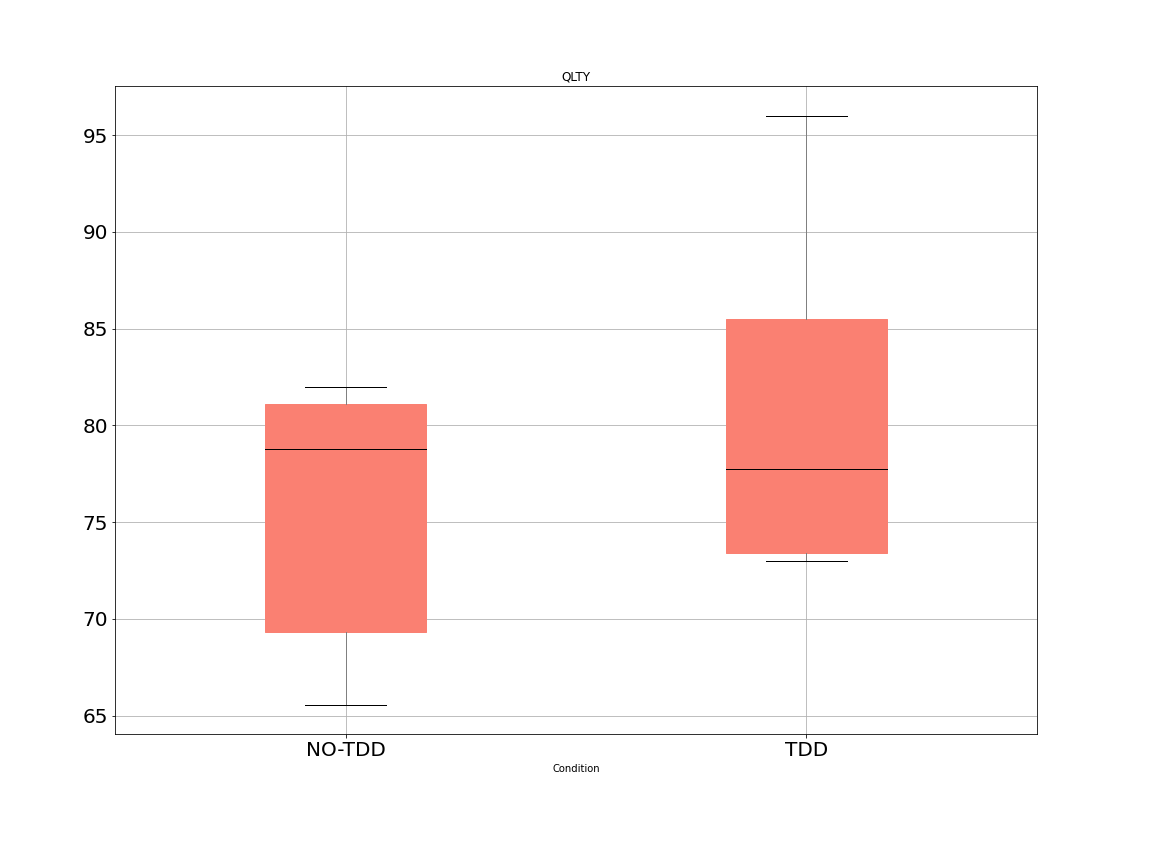
\includegraphics[width=\linewidth]{figures/box_plots/task1/QLTY.png}
        \caption{QLTY}
        \label{bp_task1_qlty}
    \end{subfigure}\hfil
        \begin{subfigure}{0.33\textwidth}
        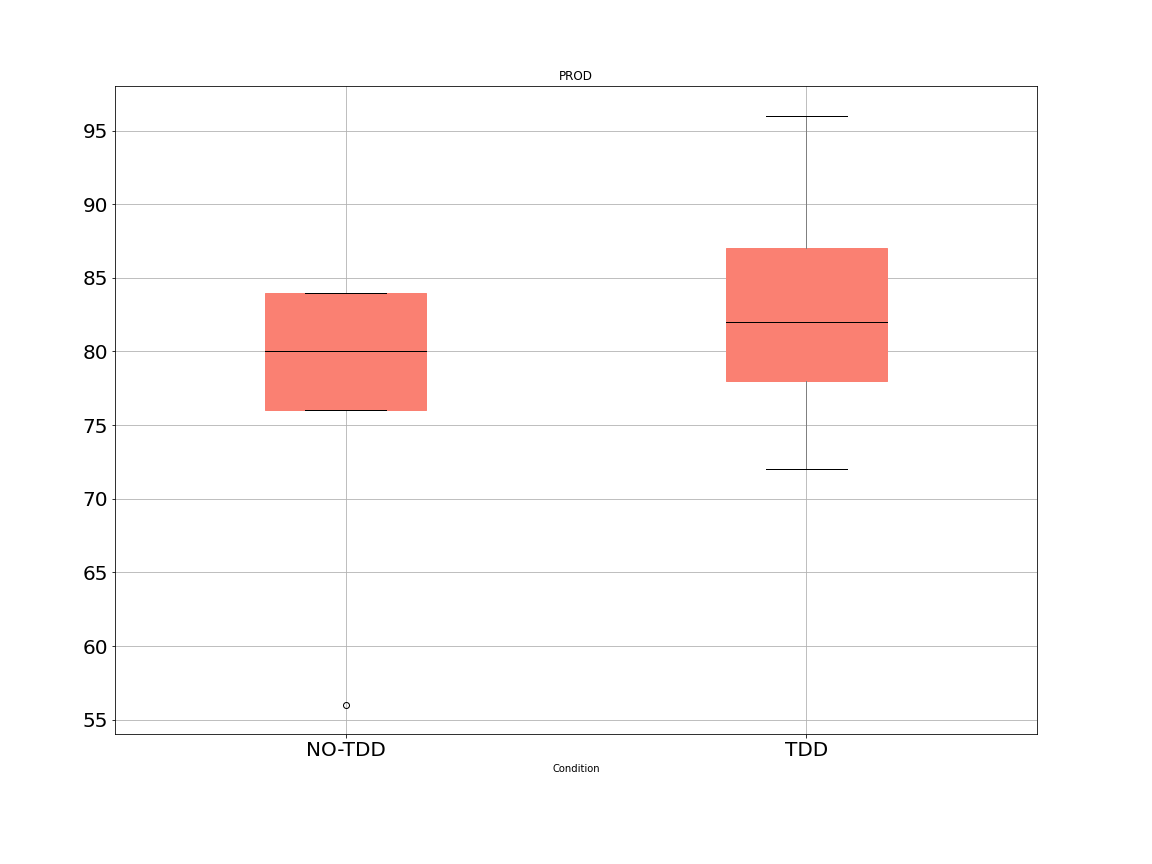
\includegraphics[width=\linewidth]{figures/box_plots/task1/PROD.png}
        \caption{PROD}
        \label{bp_task1_prod}
    \end{subfigure}\hfil
    \begin{subfigure}{0.33\textwidth}
        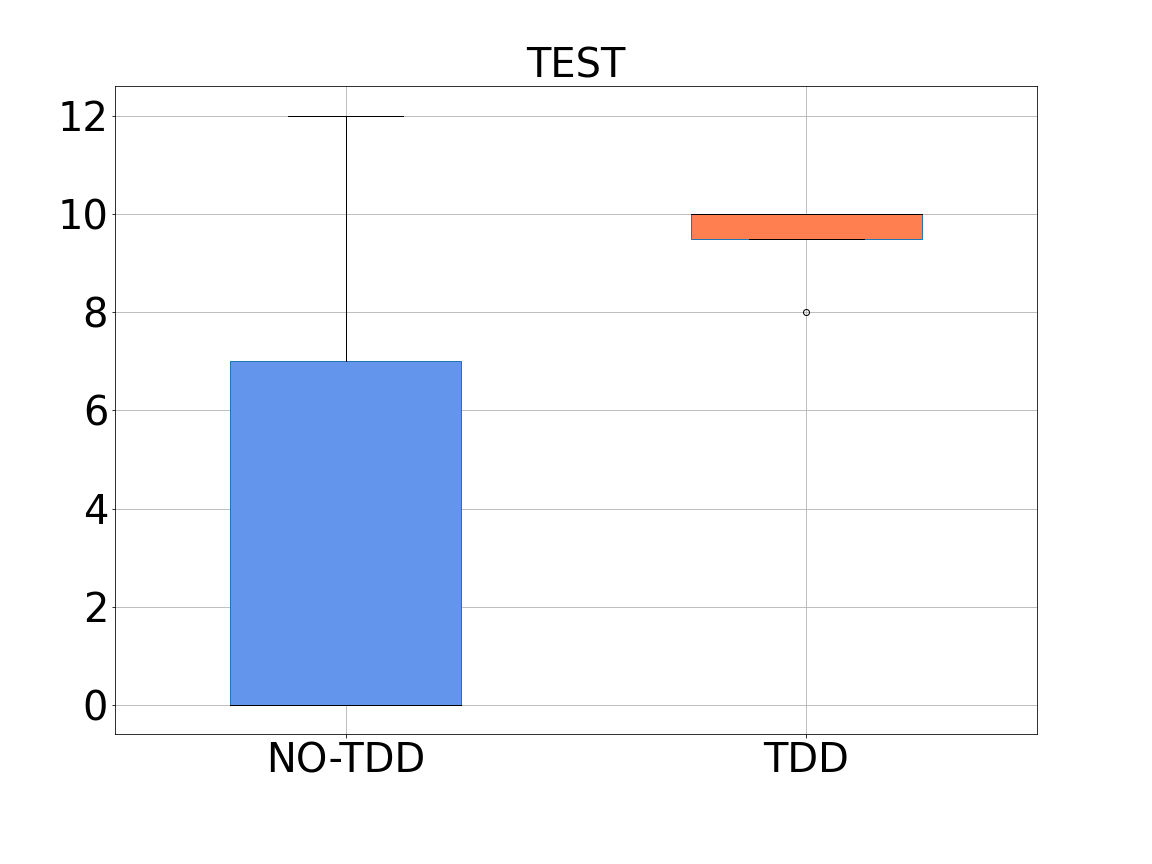
\includegraphics[width=\linewidth]{figures/box_plots/task1/TEST.png}
        \caption{TEST}
        \label{bp_task1_test}
    \end{subfigure}

    \medskip
    \begin{subfigure}{0.33\textwidth}
        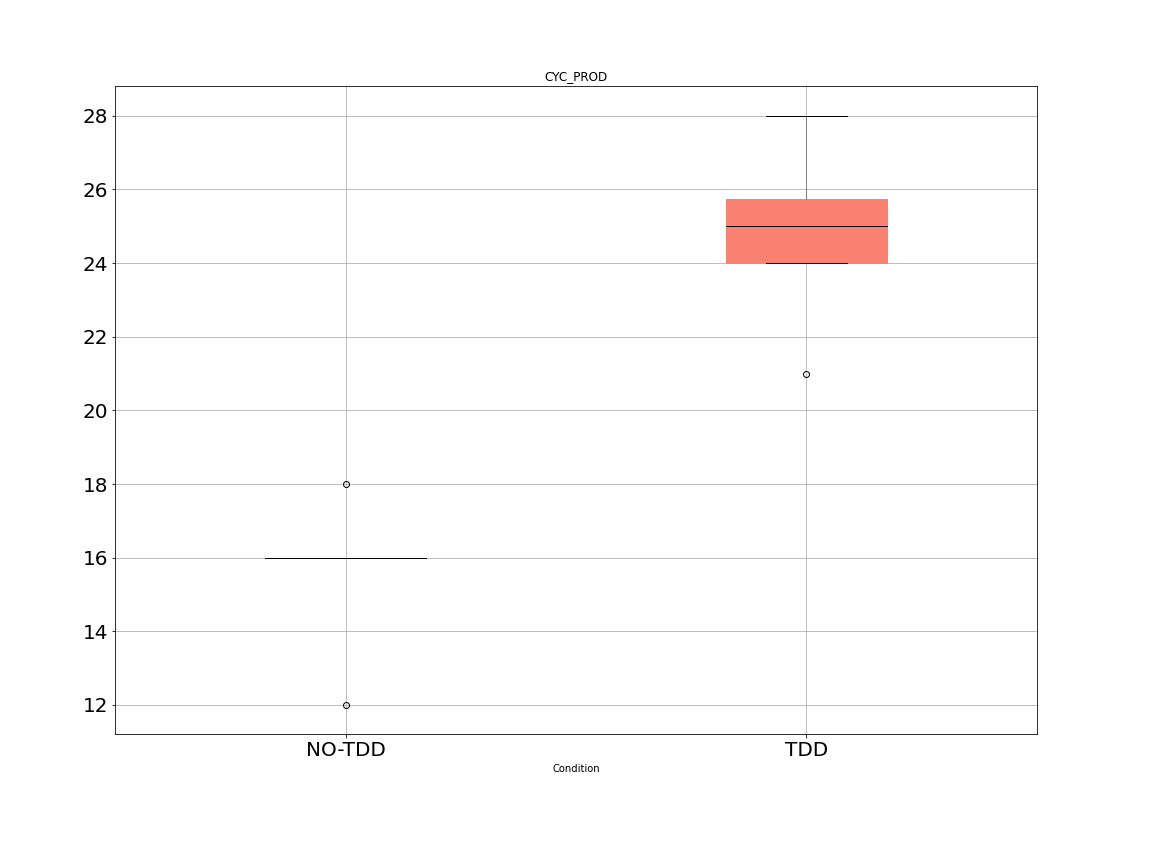
\includegraphics[width=\linewidth]{figures/box_plots/task1/CYC.png}
        \caption{CYC}
        \label{bp_task1_cyc}
    \end{subfigure}\hfil
    \begin{subfigure}{0.33\textwidth}
        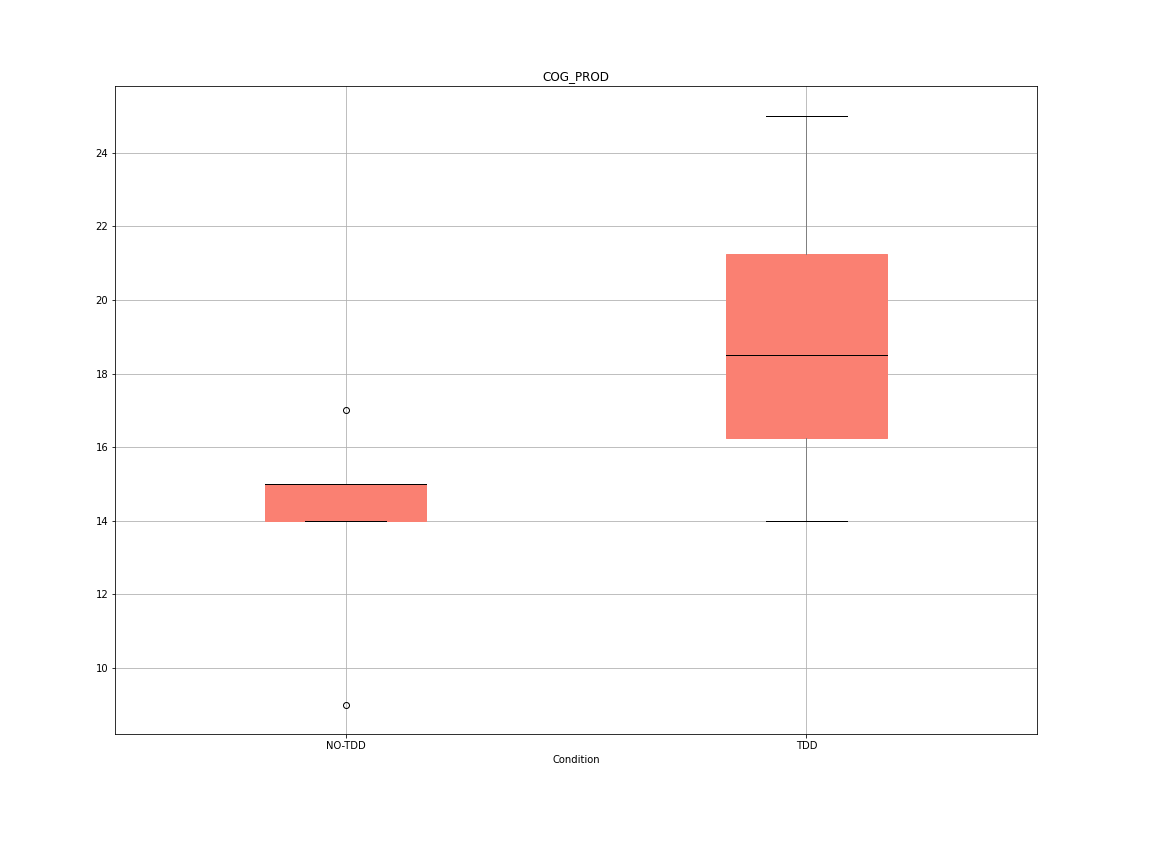
\includegraphics[width=\linewidth]{figures/box_plots/task1/COG.png}
        \caption{COG}
        \label{bp_task1_cog}
    \end{subfigure}\hfil
    \begin{subfigure}{0.33\textwidth}
        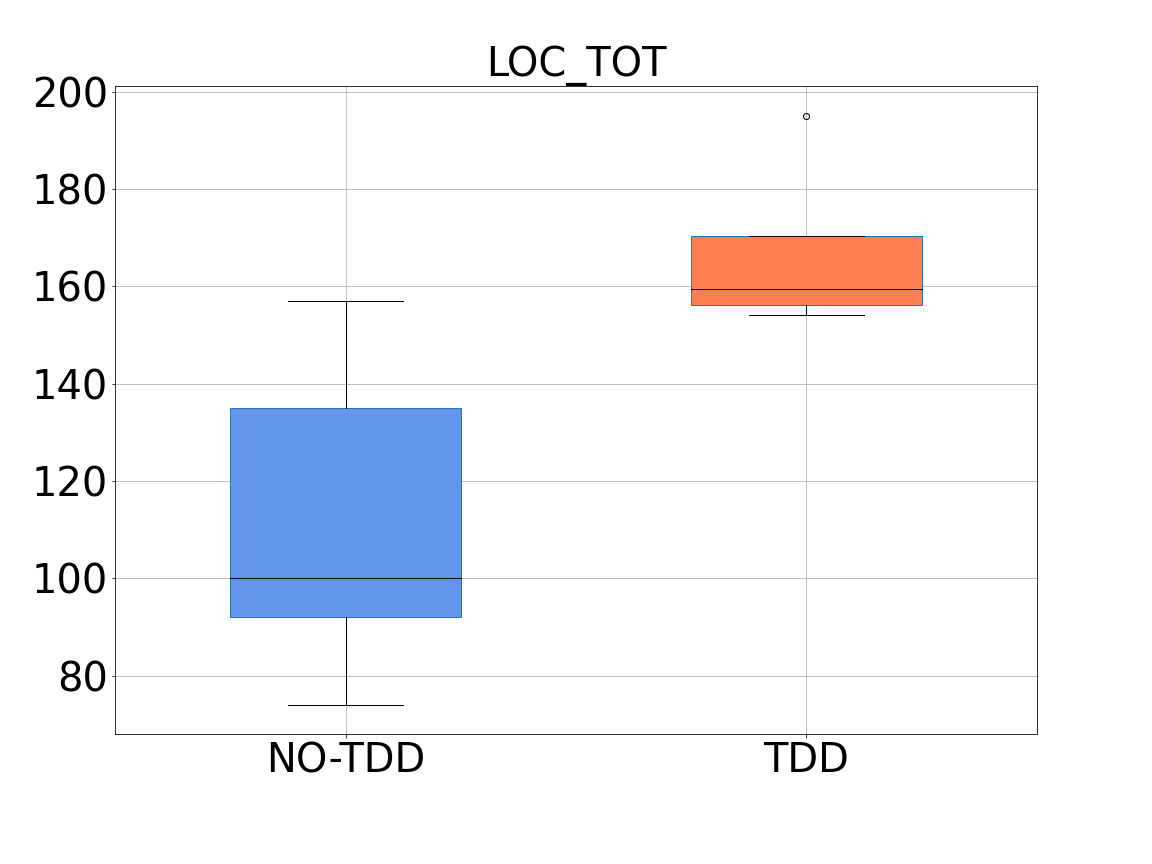
\includegraphics[width=\linewidth]{figures/box_plots/task1/LOC.png}
        \caption{LOC}
        \label{bp_task1_loc}
    \end{subfigure}
    \caption{Box plots for task 1, \textit{IntelligentOffice}.}
    \label{box_plots_task1}
\end{figure}



\begin{table}[!h]
    \begin{center} 
        \begin{tabular}{ |p{2cm}||p{1.6cm}|p{1.6cm}|p{1.6cm}|p{1.6cm}|p{1.6cm}|}
            \hline
                \multicolumn{6}{|c|}{Task 2 - TDD} \\
            \hline
                Metric & Min & Max & Mean & Median & Std\\
            \hline
                QLTY & 50 & 100 & 84.44 & 100 & 22.70 \\
                PROD & 8 & 100 & 38.6 & 21 & 37.35 \\
                TEST & 0 & 13 & 5.4 & 3 & 5.12 \\
                CYC & 9 & 19 & 12 & 10 & 4.06 \\
                COG & 2 & 40 & 12.8 & 4.0 & 15.91 \\
                LOC & 80 & 203 & 128 & 115 & 45.61 \\
            \hline
        \end{tabular}
        \caption{\label{tab_dv_t2_tdd}Dependent variables' statistics in task 2 for the \tdd group}
    \end{center}
\end{table}

\begin{table}[!h]
    \begin{center} 
        \begin{tabular}{ |p{2cm}||p{1.6cm}|p{1.6cm}|p{1.6cm}|p{1.6cm}|p{1.6cm}|}
            \hline
                \multicolumn{6}{|c|}{Task 2 - NO-TDD} \\
            \hline
                Metric & Min & Max & Mean & Median & Std\\
            \hline
                QLTY & 74 & 94.43 & 83.07 & 81.94 & 10.17 \\
                PROD & 52 & 73 & 60.5 & 58.5 & 10.24 \\
                TEST & 5 & 12 & 9 & 9.5 & 2.94 \\
                CYC & 16 & 36 & 23.5 & 21 & 9 \\
                COG & 11 & 49 & 29 & 28 & 15.57 \\
                LOC & 178 & 260 & 207.5 & 196 & 37.11 \\
            \hline
        \end{tabular}
        \caption{\label{tab_dv_t2_notdd}Dependent variables' statistics in task 2 for the \notdd group}
    \end{center}
\end{table}

\begin{figure}[htbp]
    \centering
    \begin{subfigure}{0.33\textwidth}
        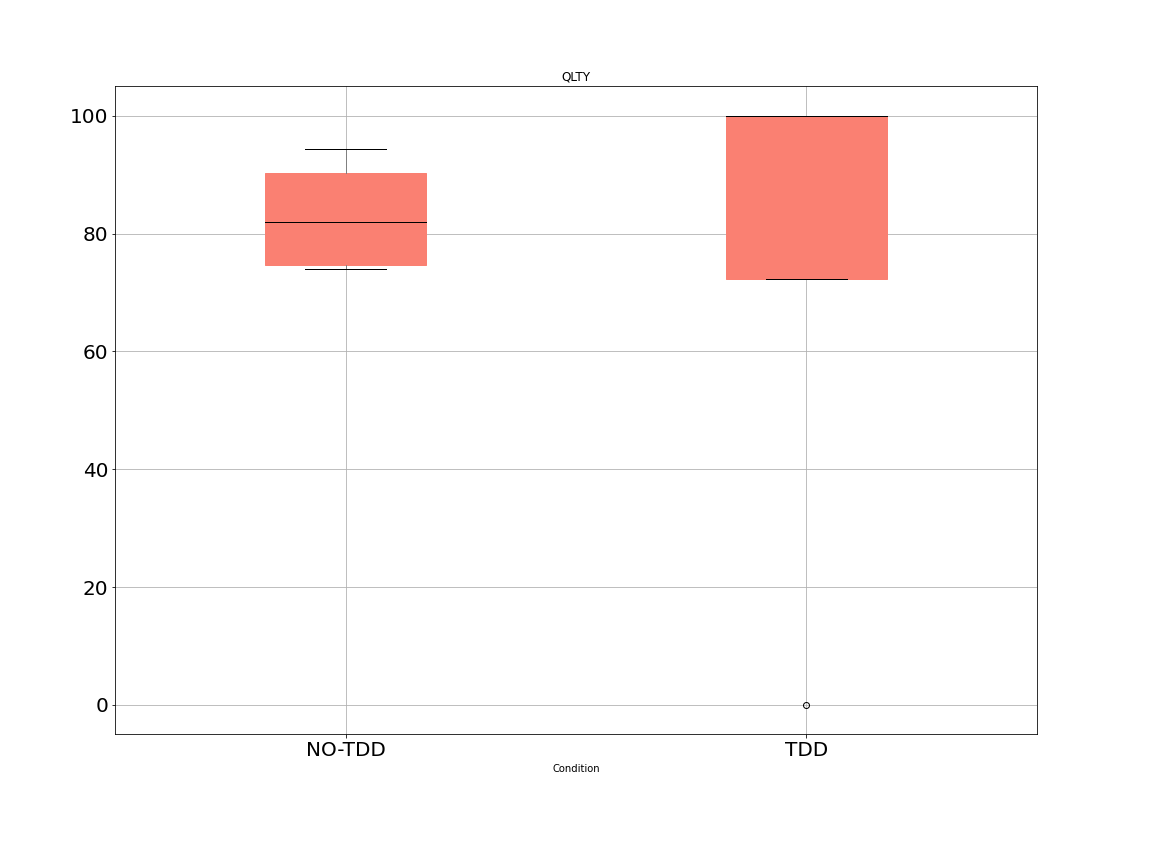
\includegraphics[width=\linewidth]{figures/box_plots/task2/QLTY.png}
        \caption{QLTY}
        \label{bp_task2_qlty}
    \end{subfigure}\hfil
        \begin{subfigure}{0.33\textwidth}
        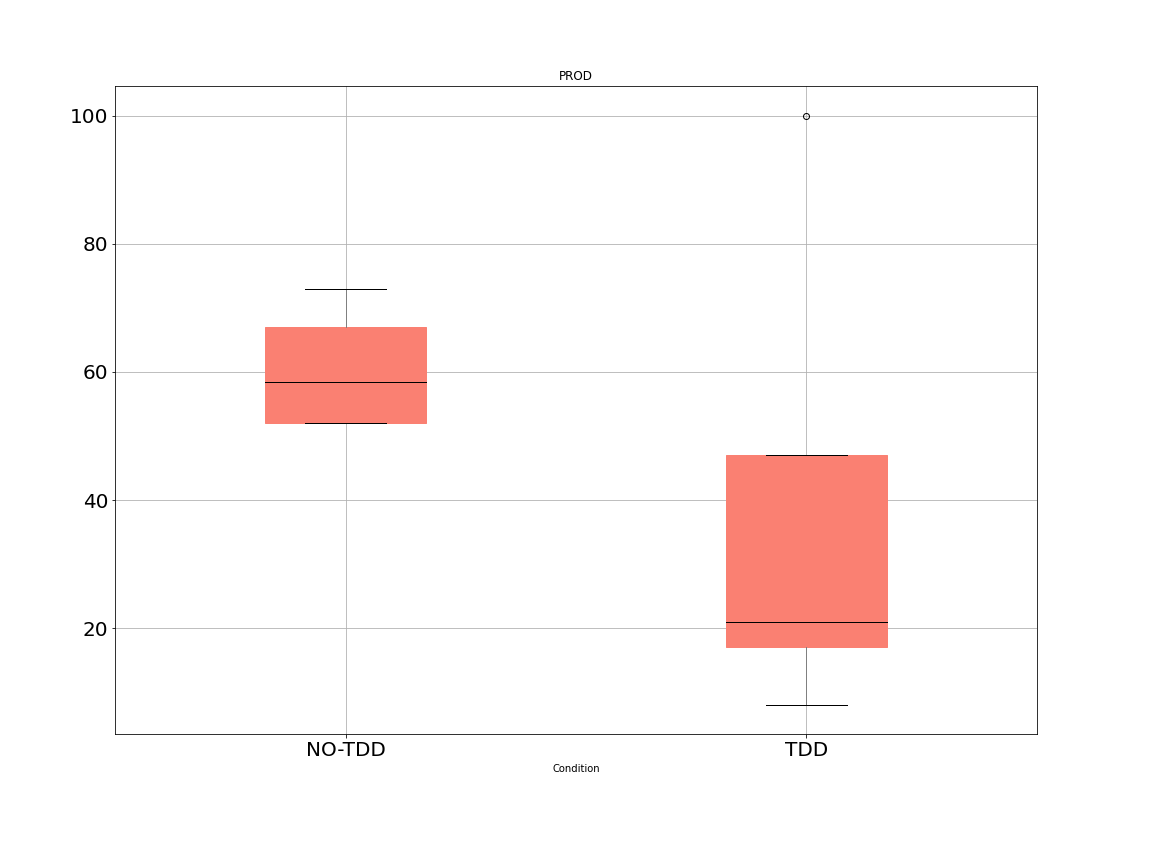
\includegraphics[width=\linewidth]{figures/box_plots/task2/PROD.png}
        \caption{PROD}
        \label{bp_task2_prod}
    \end{subfigure}\hfil
    \begin{subfigure}{0.33\textwidth}
        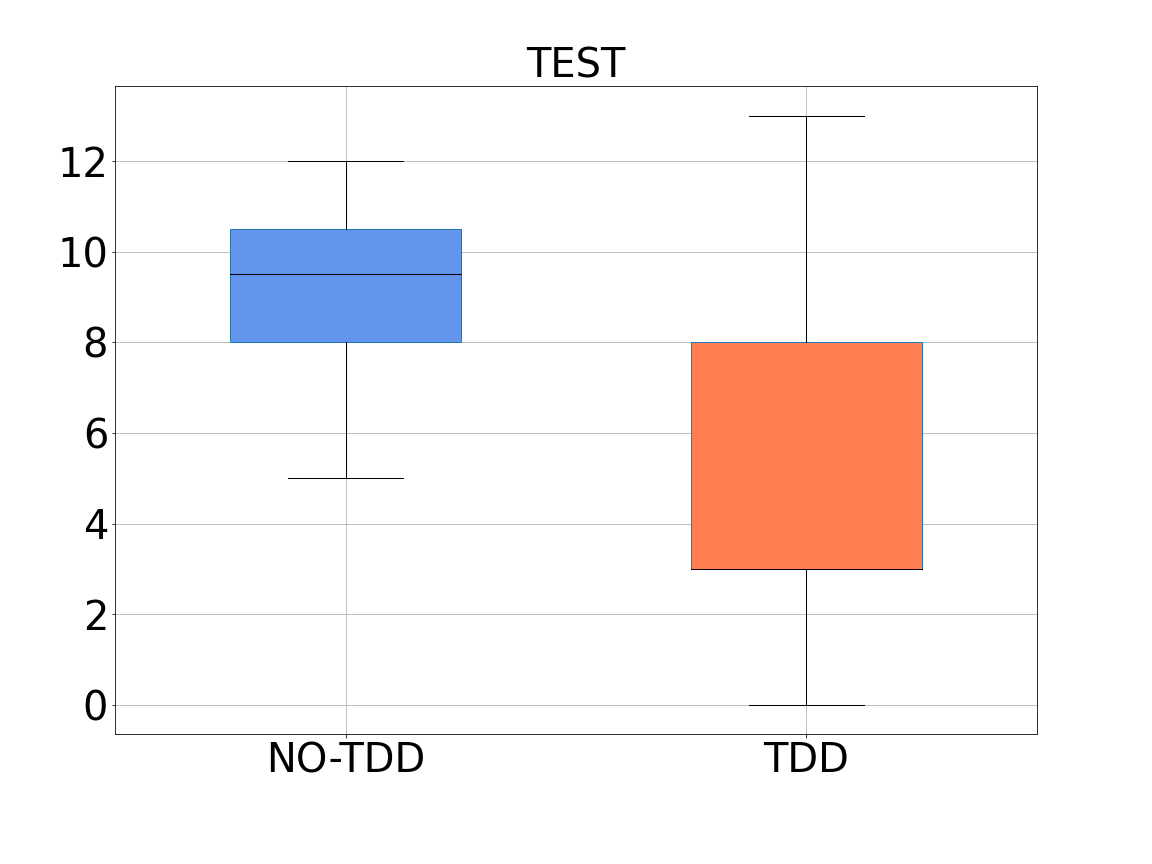
\includegraphics[width=\linewidth]{figures/box_plots/task2/TEST.png}
        \caption{TEST}
        \label{bp_task2_test}
    \end{subfigure}

    \medskip
    \begin{subfigure}{0.33\textwidth}
        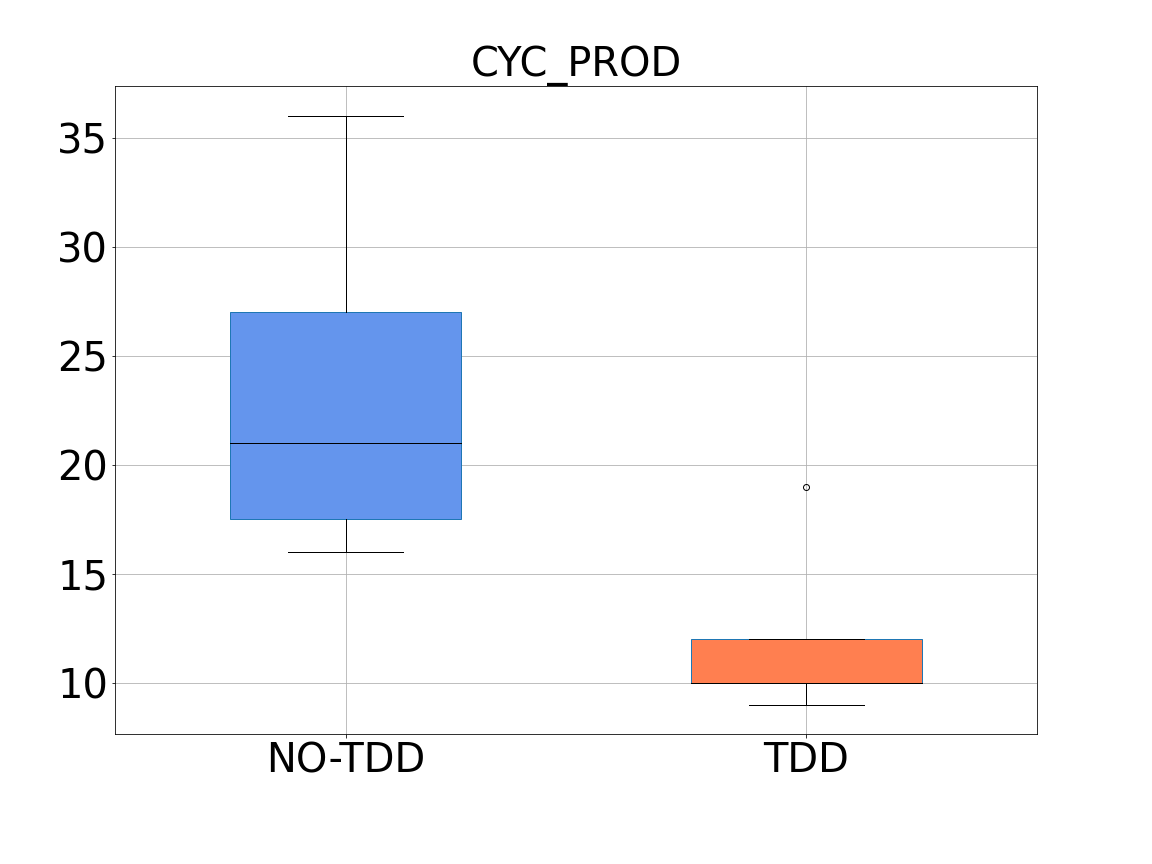
\includegraphics[width=\linewidth]{figures/box_plots/task2/CYC.png}
        \caption{CYC}
        \label{bp_task2_cyc}
    \end{subfigure}\hfil
    \begin{subfigure}{0.33\textwidth}
        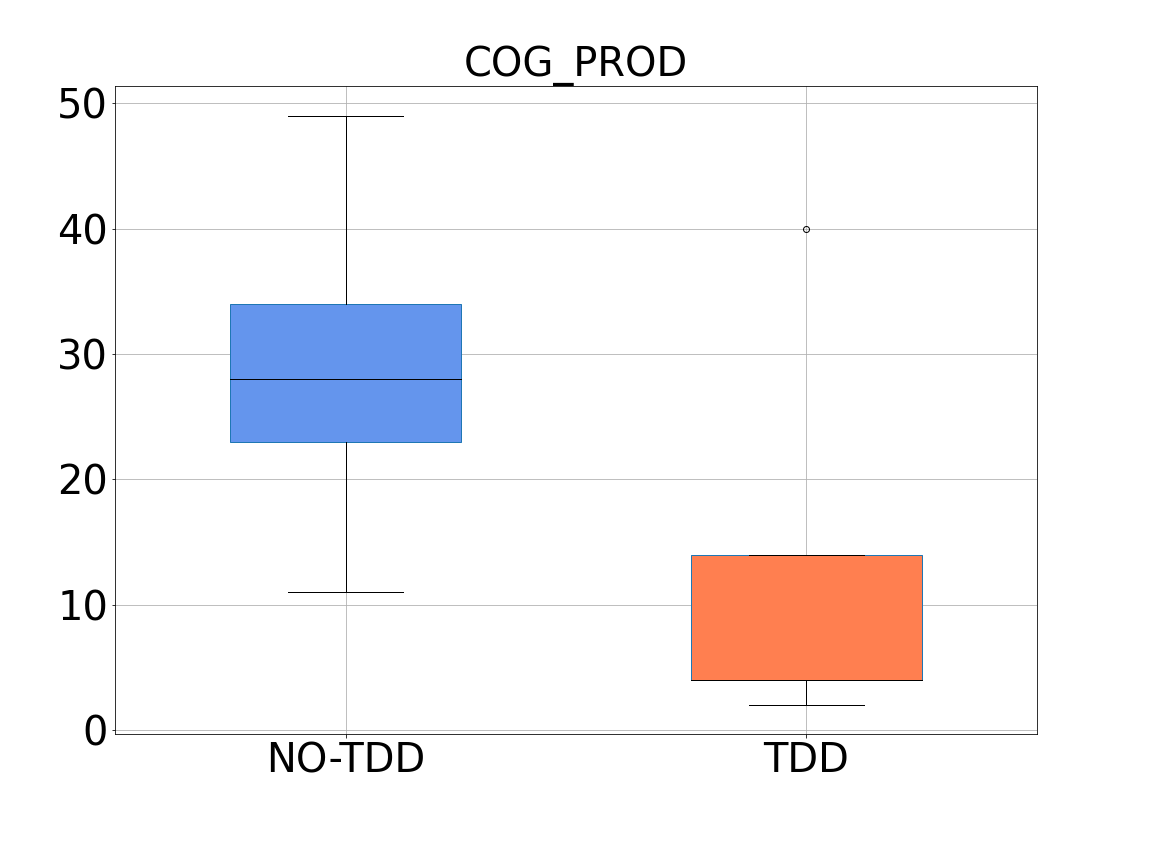
\includegraphics[width=\linewidth]{figures/box_plots/task2/COG.png}
        \caption{COG}
        \label{bp_task2_cog}
    \end{subfigure}\hfil
    \begin{subfigure}{0.33\textwidth}
        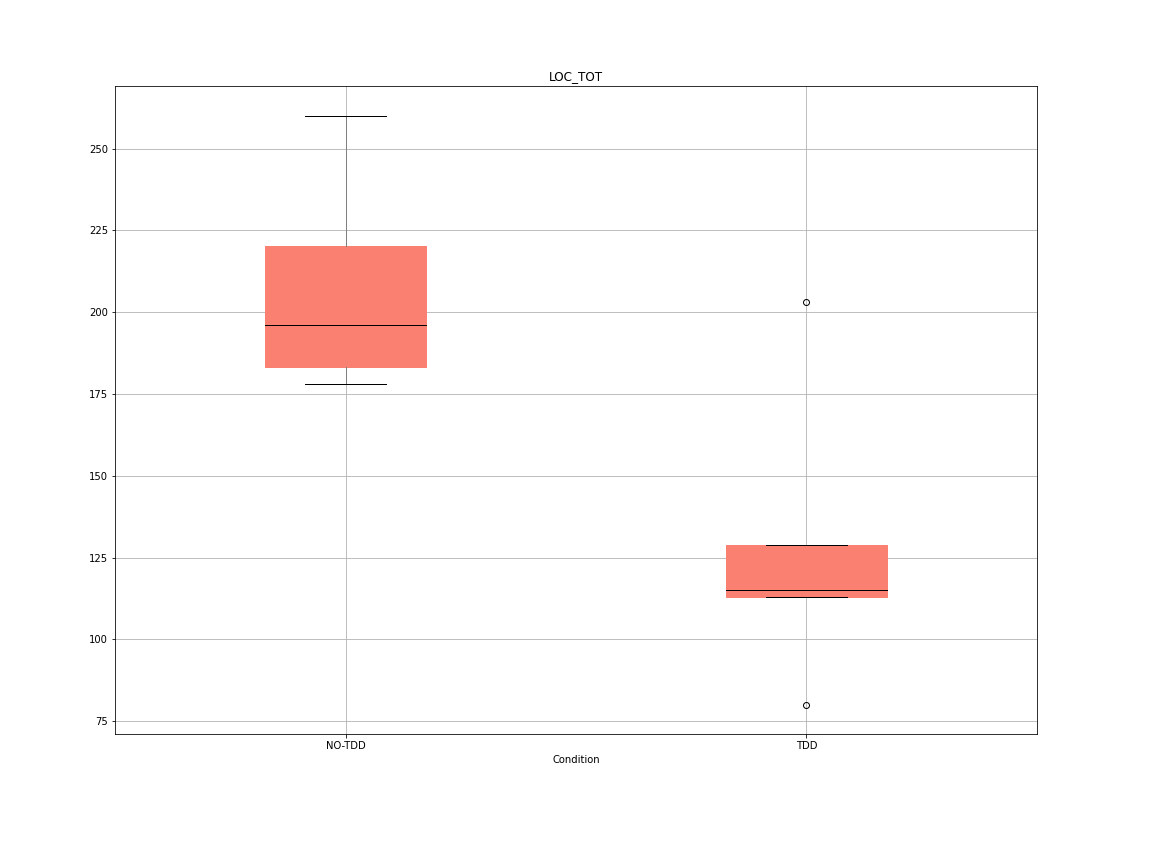
\includegraphics[width=\linewidth]{figures/box_plots/task2/LOC.png}
        \caption{LOC}
        \label{bp_task2_loc}
    \end{subfigure}
    \caption{Box plots for task 2, \textit{CleaningRobot}.}
    \label{box_plots_task2}
\end{figure}



\begin{table}[!h]
    \begin{center} 
        \begin{tabular}{ |p{2cm}||p{1.6cm}|p{1.6cm}|p{1.6cm}|p{1.6cm}|p{1.6cm}|}
            \hline
                \multicolumn{6}{|c|}{Task 1 \& 2 - TDD} \\
            \hline
                Metric & Min & Max & Mean & Median & Std\\
            \hline
                QLTY & 50 & 100 & 82.97 & 82 & 17.43 \\
                PROD & 8 & 100 & 58.33 & 72 & 35.76 \\
                TEST & 0 & 13 & 7.22 & 8 & 4.26 \\
                CYC & 9 & 28 & 17.66 & 19 & 7.51 \\
                COG & 2 & 40 & 15.55 & 14 & 12.06 \\
                LOC & 80 & 203 & 145.33 & 154 & 39.97 \\
            \hline
        \end{tabular}
        \caption{\label{tab_dv_t1_2_tdd}Dependent variables' statistics in tasks 1 and 2 for the \tdd group}
    \end{center}
\end{table}

\begin{table}[!h]
    \begin{center} 
        \begin{tabular}{ |p{2cm}||p{1.6cm}|p{1.6cm}|p{1.6cm}|p{1.6cm}|p{1.6cm}|}
            \hline
                \multicolumn{6}{|c|}{Task 1 \& 2 - NO-TDD} \\
            \hline
                Metric & Min & Max & Mean & Median & Std\\
            \hline
                QLTY & 65.55 & 94.43 & 78.78 & 78.77 & 9.11 \\
                PROD & 52 & 84 & 69.11 & 73 & 13.22 \\
                TEST & 0 & 12 & 6.11 & 7.0 & 5.08 \\
                CYC & 12 & 36 & 19.11 & 16 & 7.07 \\
                COG & 9 & 49 & 20.66 & 15 & 12.56 \\
                LOC & 74 & 260 & 154.22 & 157 & 60.32 \\
            \hline
        \end{tabular}
        \caption{\label{tab_dv_t1_2_notdd}Dependent variables' statistics in tasks 1 and 2 for the \notdd group}
    \end{center}
\end{table}

\begin{figure}[htbp]
    \centering
    \begin{subfigure}{0.33\textwidth}
        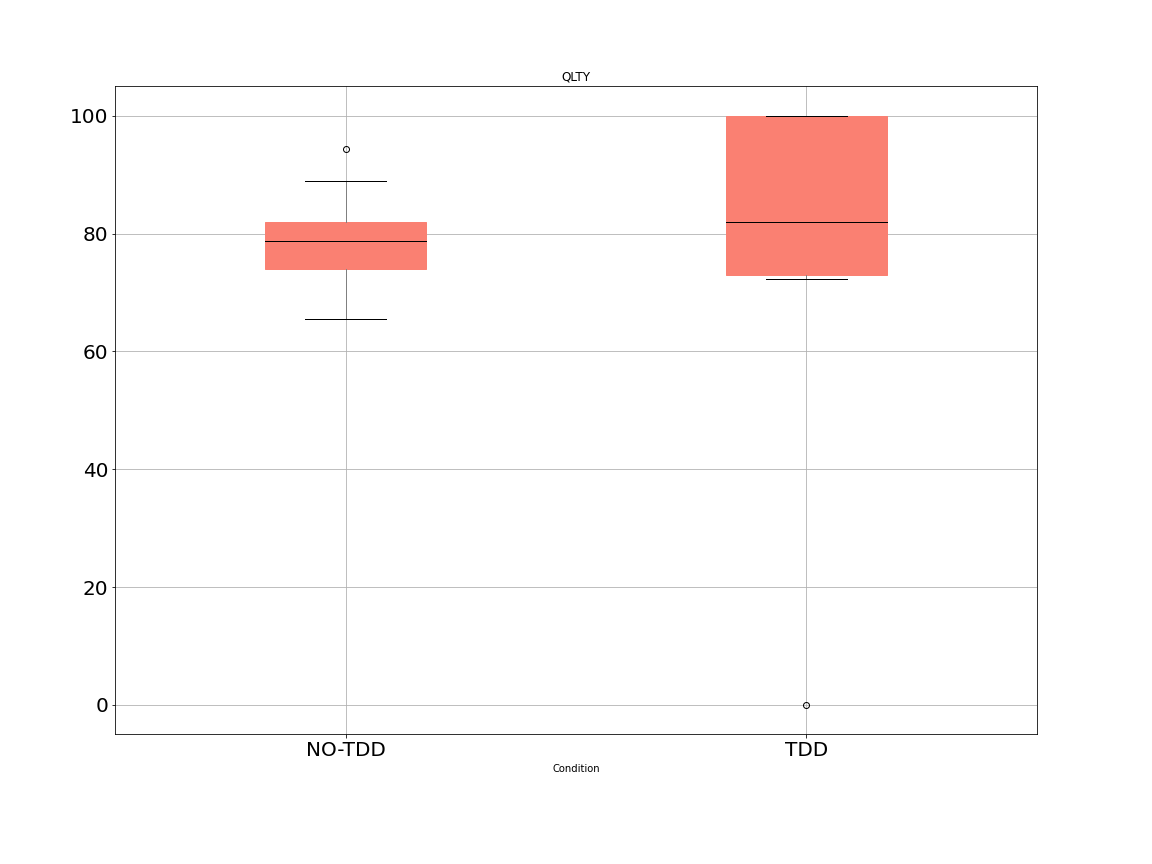
\includegraphics[width=\linewidth]{figures/box_plots/task1_2/QLTY.png}
        \caption{QLTY}
        \label{bp_task1_2_qlty}
    \end{subfigure}\hfil
        \begin{subfigure}{0.33\textwidth}
        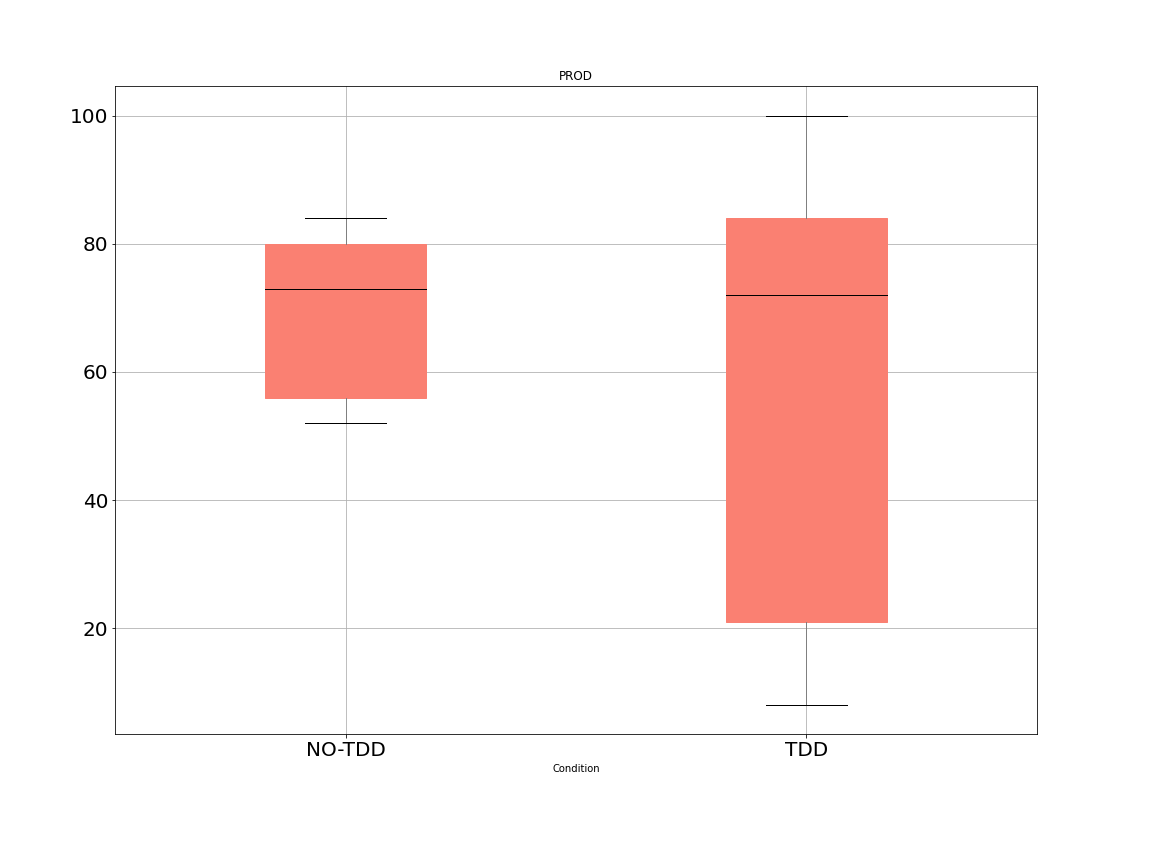
\includegraphics[width=\linewidth]{figures/box_plots/task1_2/PROD.png}
        \caption{PROD}
        \label{bp_task1_2_prod}
    \end{subfigure}\hfil
    \begin{subfigure}{0.33\textwidth}
        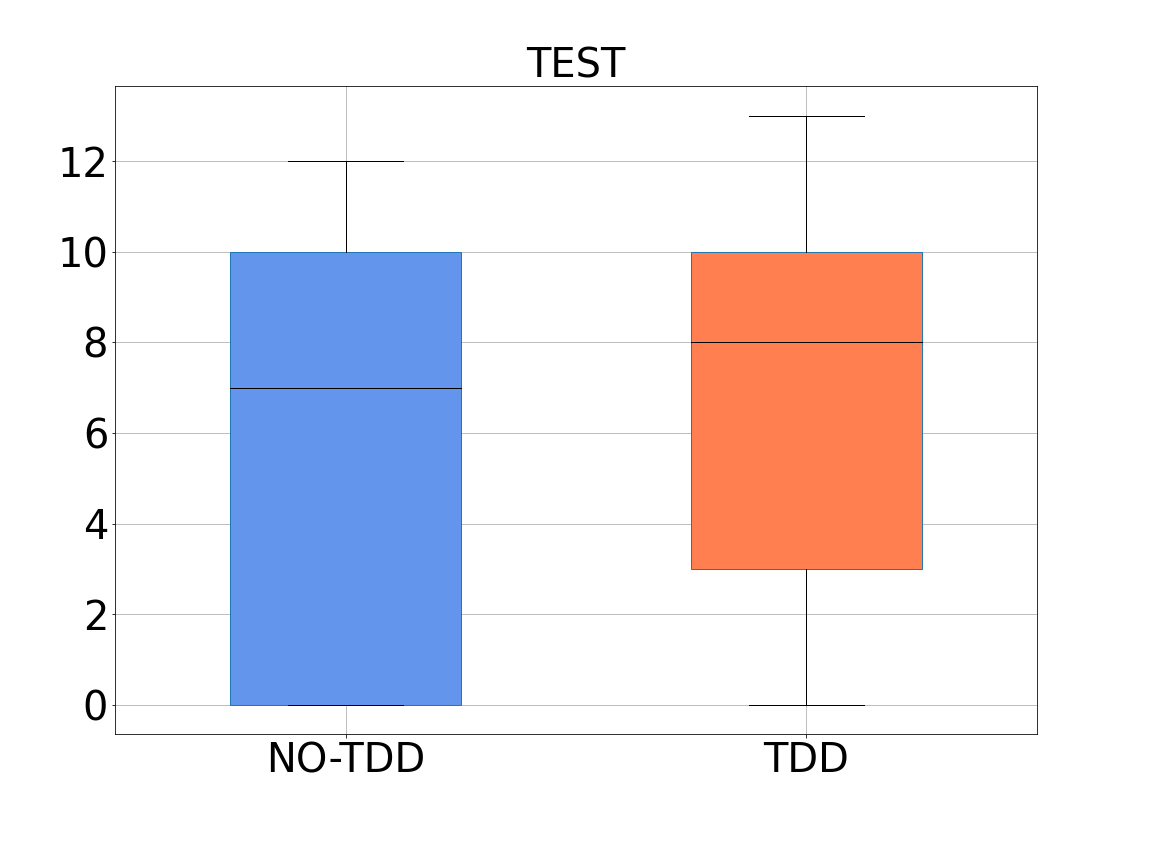
\includegraphics[width=\linewidth]{figures/box_plots/task1_2/TEST.png}
        \caption{TEST}
        \label{bp_task1_2_test}
    \end{subfigure}

    \medskip
    \begin{subfigure}{0.33\textwidth}
        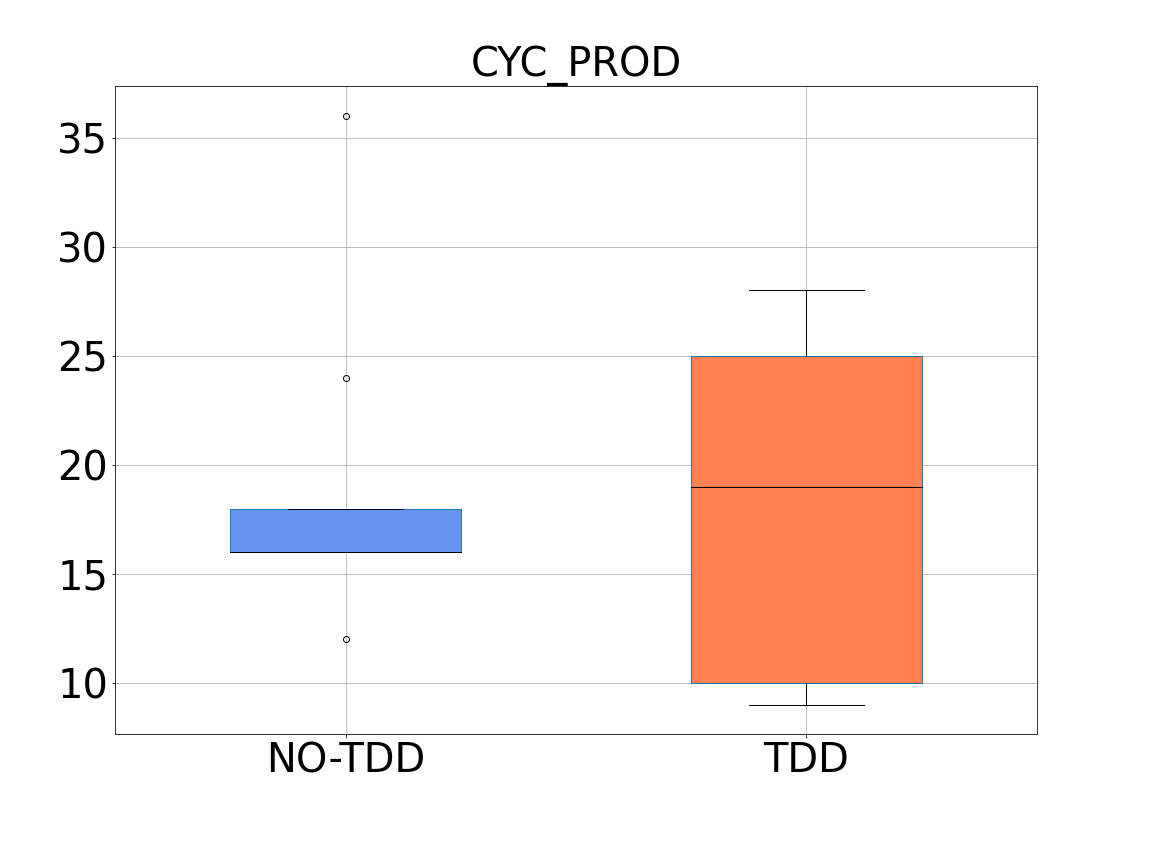
\includegraphics[width=\linewidth]{figures/box_plots/task1_2/CYC.png}
        \caption{CYC}
        \label{bp_task1_2_cyc}
    \end{subfigure}\hfil
    \begin{subfigure}{0.33\textwidth}
        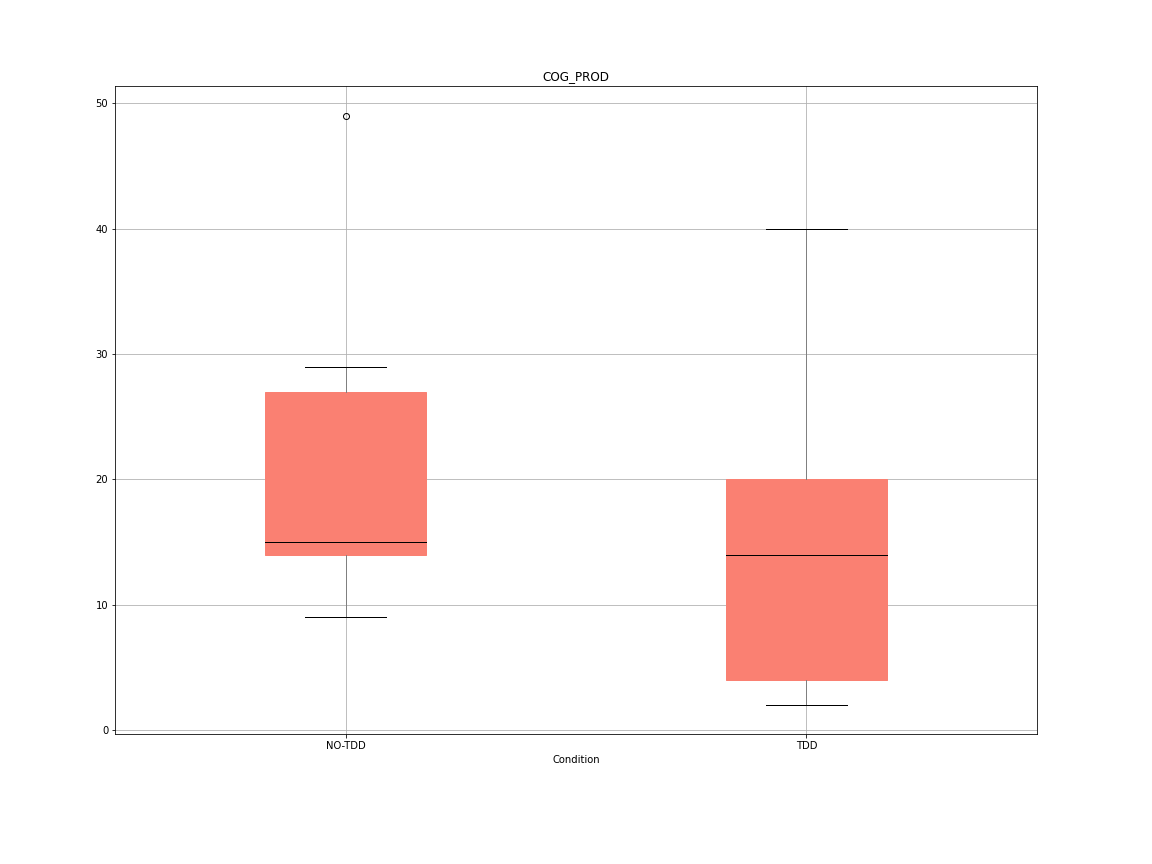
\includegraphics[width=\linewidth]{figures/box_plots/task1_2/COG.png}
        \caption{COG}
        \label{bp_task1_2_cog}
    \end{subfigure}\hfil
    \begin{subfigure}{0.33\textwidth}
        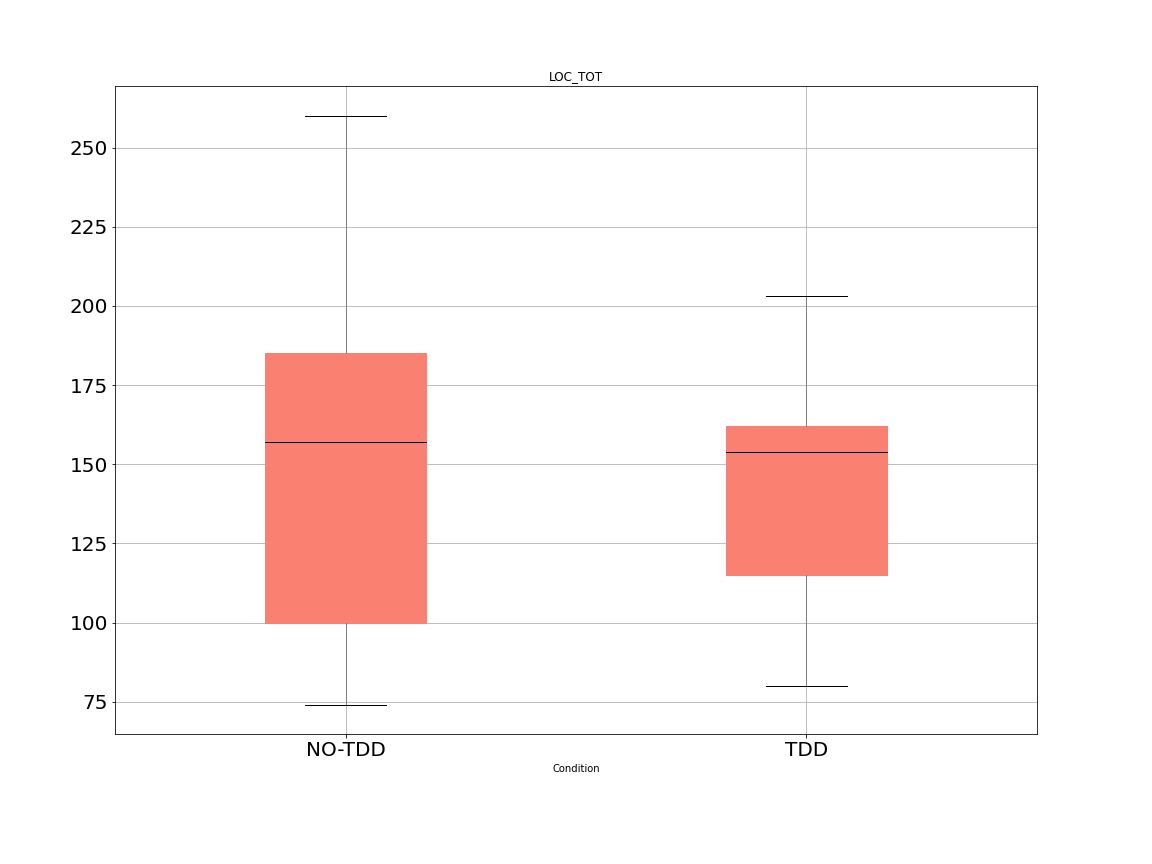
\includegraphics[width=\linewidth]{figures/box_plots/task1_2/LOC.png}
        \caption{LOC}
        \label{bp_task1_2_loc}
    \end{subfigure}
    \caption{Aggregated box plots for tasks 1 and 2.}
    \label{box_plots_task1_2}
\end{figure}



\begin{table}[!h]
    \begin{center} 
        \begin{tabular}{ |p{2cm}||p{1.6cm}|p{1.6cm}|p{1.6cm}|p{1.6cm}|p{1.6cm}|}
            \hline
                \multicolumn{6}{|c|}{Task 3 - TDD} \\
            \hline
                Metric & Min & Max & Mean & Median & Std\\
            \hline
                QLTY & 85 & 100 & 95 & 100 & 7.07 \\
                PROD & 83.33 & 100 & 93.33 & 100 & 9.13 \\
                TEST & 7 & 18 & 11.6 & 12 & 4.15 \\
                CYC & 15 & 30 & 22.6 & 20 & 6.58 \\
                COG & 18 & 34 & 25.8 & 25 & 7.08 \\
                LOC & 150 & 232 & 187 & 175 & 36.15 \\
            \hline
        \end{tabular}
        \caption{\label{tab_dv_t3_tdd}Dependent variables' statistics in task 3 for the \tdd group}
    \end{center}
\end{table}

\begin{table}[!h]
    \begin{center} 
        \begin{tabular}{ |p{2cm}||p{1.6cm}|p{1.6cm}|p{1.6cm}|p{1.6cm}|p{1.6cm}|}
            \hline
                \multicolumn{6}{|c|}{Task 3 - NO-TDD} \\
            \hline
                Metric & Min & Max & Mean & Median & Std\\
            \hline
                QLTY & 80 & 100 & 86.25 & 82.5 & 9.46 \\
                PROD & 75 & 100 & 83.33 & 79.16 & 11.78 \\
                TEST & 0 & 11 & 4.5 & 3.5 & 5.44 \\
                CYC & 16 & 23 & 19.5 & 19.5 & 2.88 \\
                COG & 19 & 25 & 21 & 20 & 2.70 \\
                LOC & 93 & 164 & 125.5 & 122.5 & 36.82 \\
            \hline
        \end{tabular}
        \caption{\label{tab_dv_t3_notdd}Dependent variables' statistics in task 3 for the \notdd group}
    \end{center}
\end{table}

\begin{figure}[htbp]
    \centering
    \begin{subfigure}{0.33\textwidth}
        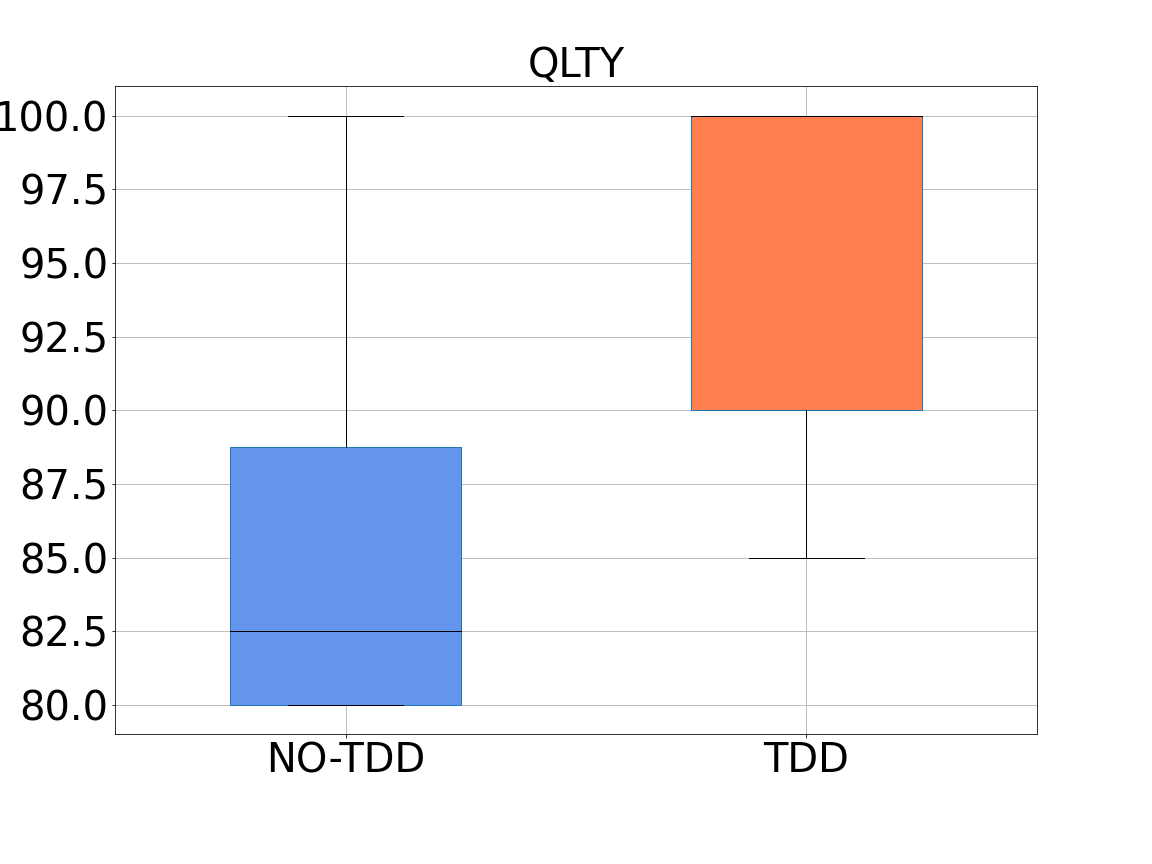
\includegraphics[width=\linewidth]{figures/box_plots/task3/QLTY.png}
        \caption{QLTY}
        \label{bp_task3_qlty}
    \end{subfigure}\hfil
        \begin{subfigure}{0.33\textwidth}
        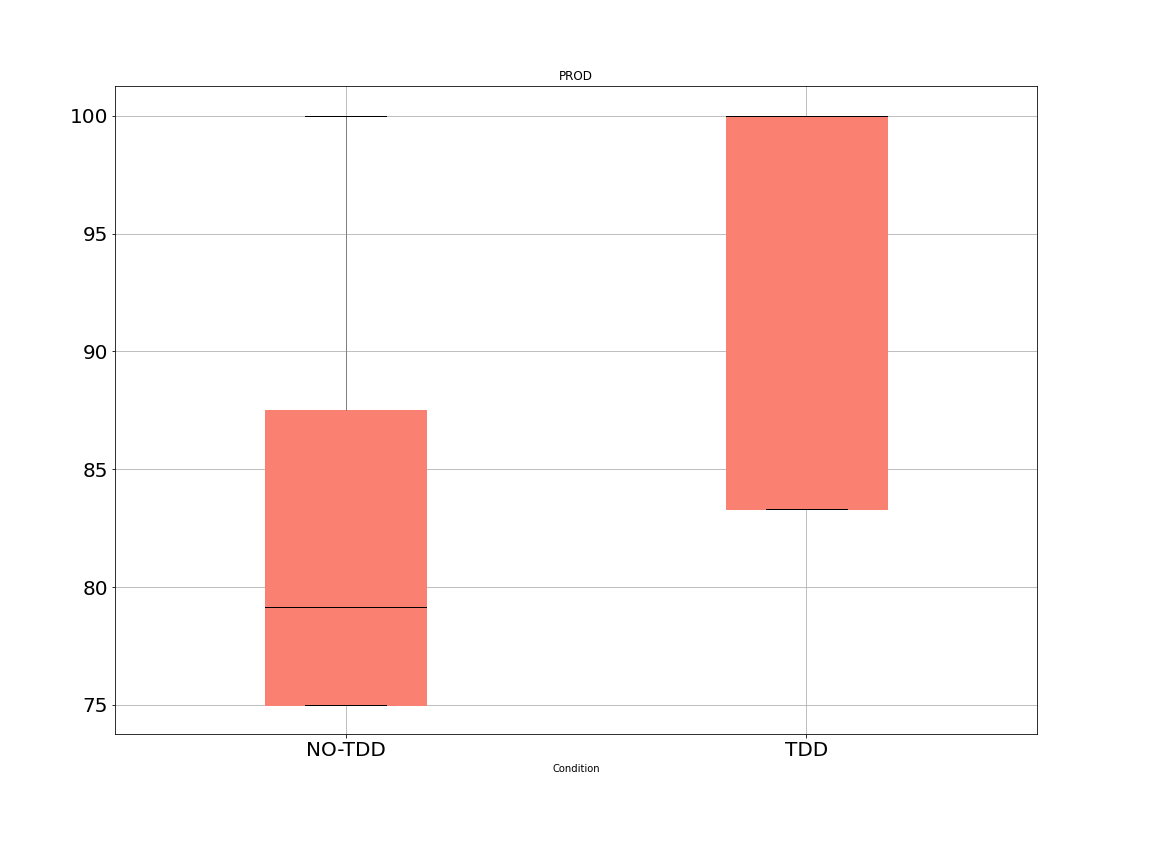
\includegraphics[width=\linewidth]{figures/box_plots/task3/PROD.png}
        \caption{PROD}
        \label{bp_task3_prod}
    \end{subfigure}\hfil
    \begin{subfigure}{0.33\textwidth}
        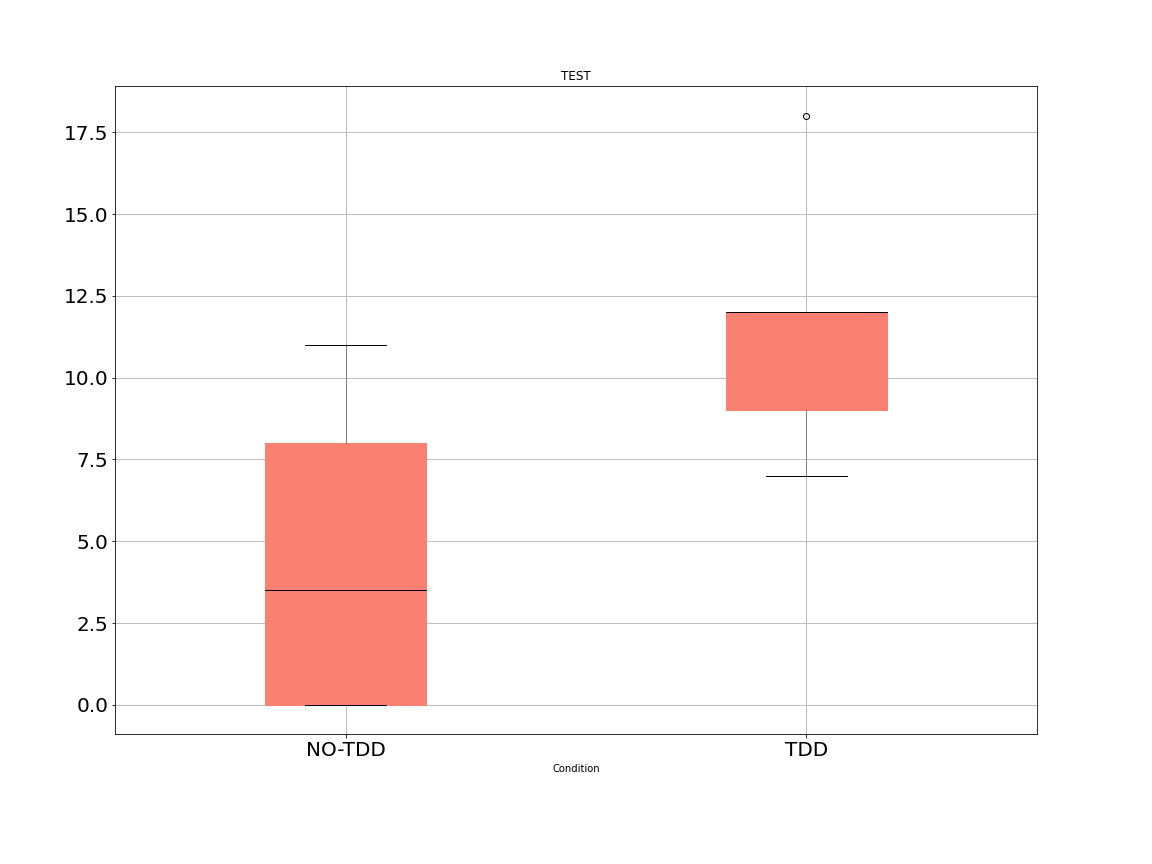
\includegraphics[width=\linewidth]{figures/box_plots/task3/TEST.png}
        \caption{TEST}
        \label{bp_task3_test}
    \end{subfigure}

    \medskip
    \begin{subfigure}{0.33\textwidth}
        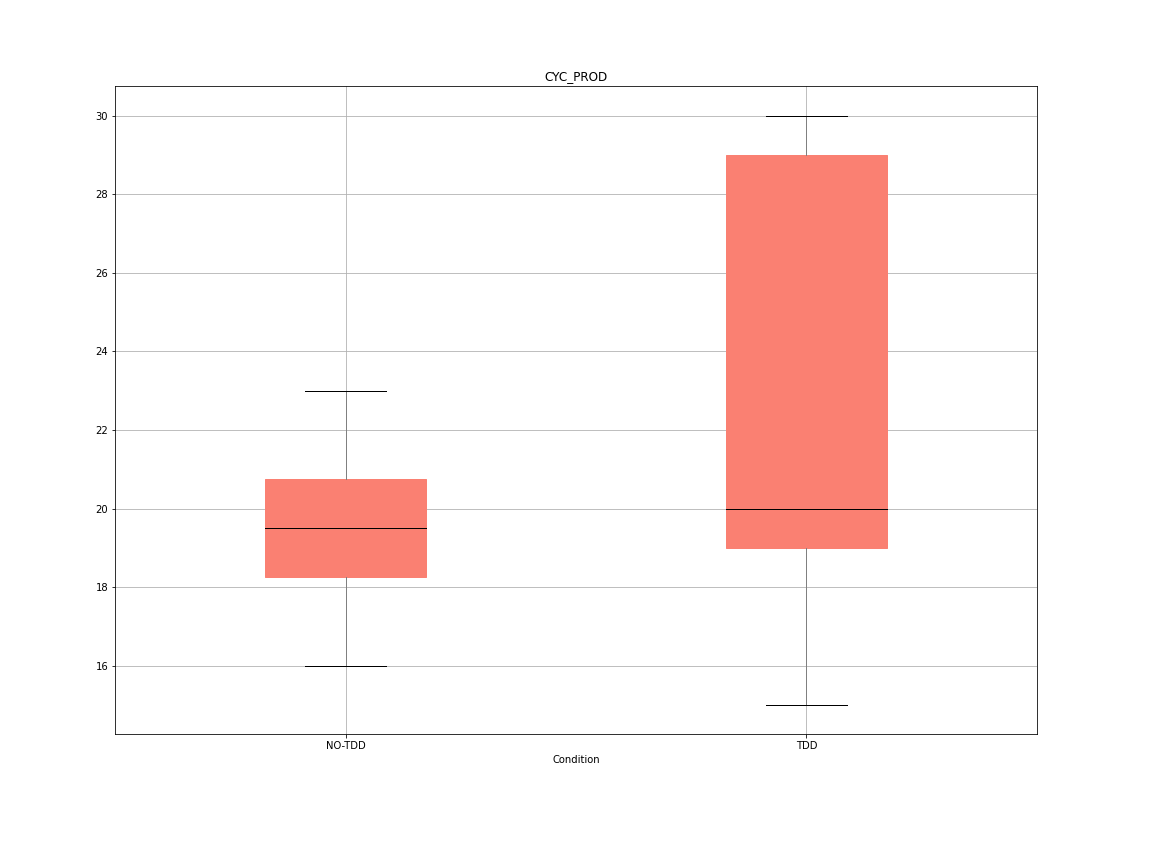
\includegraphics[width=\linewidth]{figures/box_plots/task3/CYC.png}
        \caption{CYC}
        \label{bp_task3_cyc}
    \end{subfigure}\hfil
    \begin{subfigure}{0.33\textwidth}
        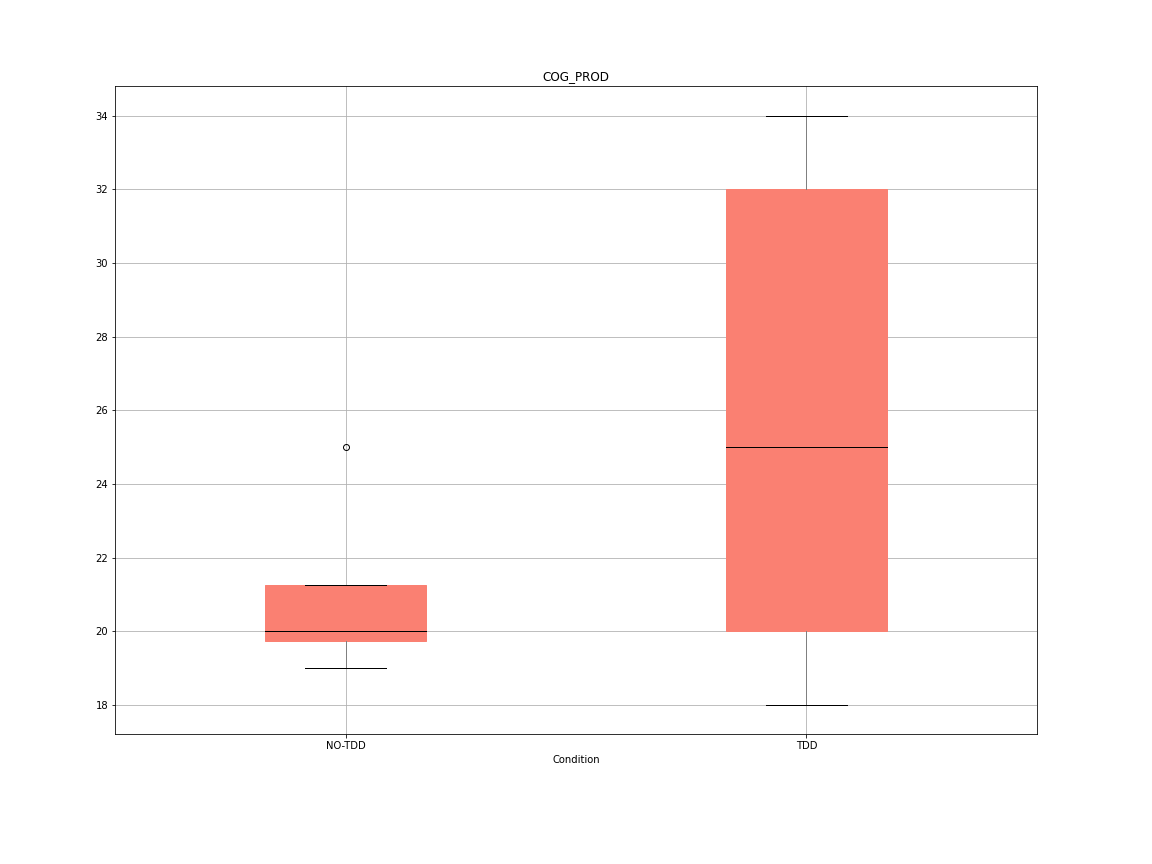
\includegraphics[width=\linewidth]{figures/box_plots/task3/COG.png}
        \caption{COG}
        \label{bp_task3_cog}
    \end{subfigure}\hfil
    \begin{subfigure}{0.33\textwidth}
        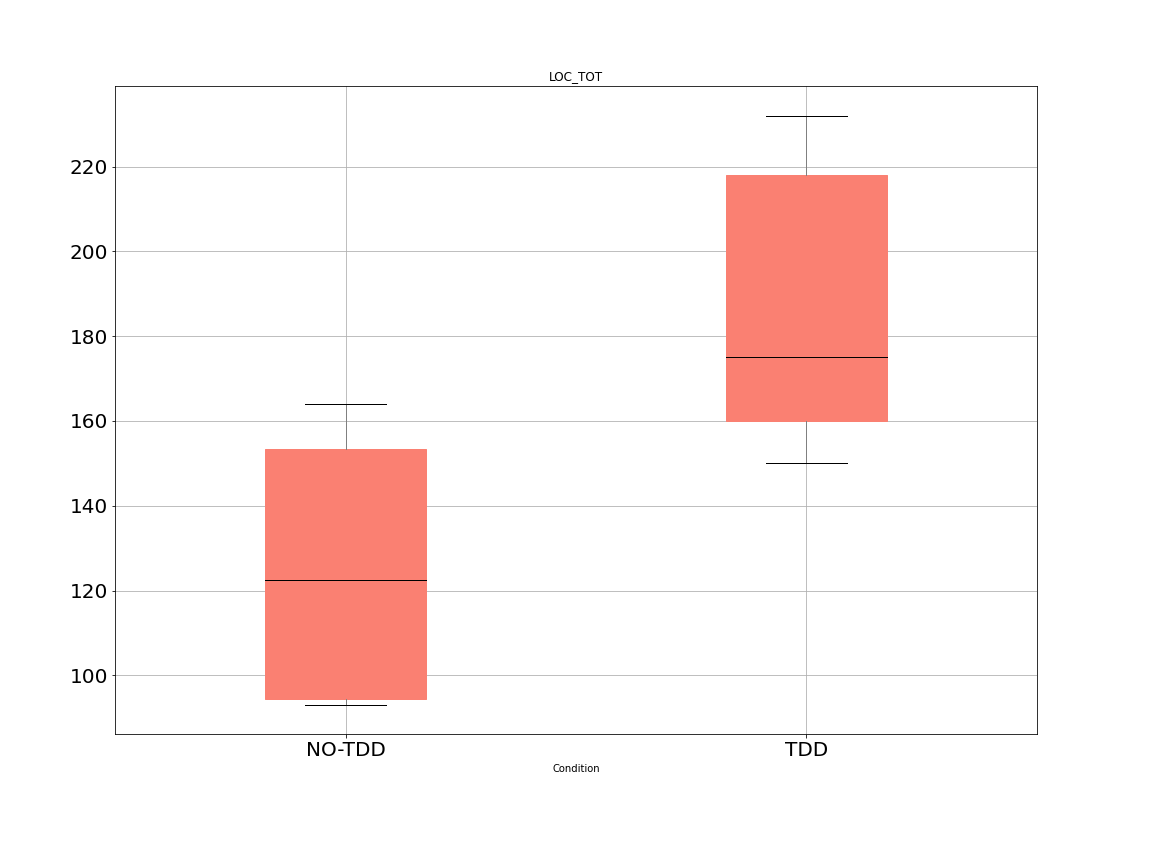
\includegraphics[width=\linewidth]{figures/box_plots/task3/LOC.png}
        \caption{LOC}
        \label{bp_task3_loc}
    \end{subfigure}
    \caption{Box plots for task 3, \textit{SmartHome}.}
    \label{box_plots_task3}
\end{figure}